\section{Algoritmo Genético}

Um \emph{algoritmo genético} é uma heurística de busca que procura
imitar a seleção natural que ocorre no processo evolucionário dos
organismos vivos.

Nessa heurística, uma população de soluções (também chamadas de
indivíduos ou fenótipos) para problemas de otimização é evoluída para
conseguir soluções melhores. Cada solução possui um conjunto de
propriedades (cromossomos ou genótipos) que podem ser mutados ou
alterados.

Os requerimentos são, tipicamente:

\begin{itemize}
\item
  uma representação genética da solução
\item
  uma função de aptidão para avaliação da solução
\end{itemize}

\subsection{O processo}

O processo é iniciado com uma população com propriedades geradas
aleatoriamente.

A iteração da heurística se da em 3 etapas:

\begin{itemize}
\item
  procriação: indivíduos são pareados e é aplicada a operação de
  cruzamento (\emph{crossover}) exemplificado na figura~\ref{fig:ga_crossover}
\item
  mutação: alguns indivíduos são selecionados e é aplicada a operação de
  mutação (\emph{mutation})
\item
  seleção: é usada a função de aptidão, que define quão boa é a solução para o problema,
  para descartar os indivíduos menos aptos restando as soluções que de fato trouxeram alguma melhora.
\end{itemize}

\begin{figure}[ht]
\centering
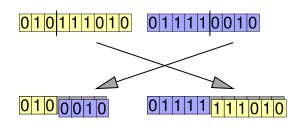
\includegraphics[width=10cm]{figuras/ga_crossover}
\caption{Cruzamento por \textit{slicing}.}\label{fig:ga_crossover}
\end{figure}

As condições mais comuns para terminação do processo são as seguintes:

\begin{itemize}
\item
  encontrada uma solução que atende os requisitos mínimos
\item
  número fixo de gerações alcançado
\item
  recursos alocados (tempo ou dinheiro) alcançados
\item
  a melhor solução alcançou um patamar estável em que mais iterações não
  produzem soluções melhores
\item
  inspeção manual
\end{itemize}

\subsection{Limitações}

As limitações mais comuns no emprego de um algoritmo genético são:

\begin{itemize}
\item
  Funções de avaliação computacionalmente caras tornam essa heurística
  ineficiente.
\item
  Não escala bem com a complexidade, isto é, quando o número de
  elementos expostos a mutação é grande o espaço de busca cresce
  exponencialmente. Por isso, na prática algoritmos genéticos são
  usados para, por exemplo, projetar uma hélice e não um motor.
\item
  A melhor solução é relativa às outras soluções, por isso o critério de
  parada não é muito claro em alguns problemas.
\item
  Em muitos problemas os algoritmos genéticos tendem a convergir para
  um ótimo local ou as vezes pontos arbitrários em vez do ótimo global.
\item
  É difícil aplicar algoritmos genéticos para conjunto de dados
  dinâmicos. Pois as soluções podem começar a convergir para um conjunto
  de dados que já não é mais válido.
\item
  Algoritmos genéticos não conseguem resolver eficientemente problemas
  em que a avaliação é binária (certo/errado), como em problemas de
  decisão. Nesse caso buscas aleatórias convergem tão rápido quanto essa
  heurística.
\item
  Para problemas mais específicos existem outras heurísticas que
  encontram a solução mais rapidamente.
\end{itemize}

\subsection{Pseudo código de um Algoritmo Genético}

%\begin{lstlisting}
\begin{algorithm}[H]
\SetKwBlock{Procedimento}{Procedimento}{fim}

%Algorithm: GA(n, \ki, \mu)
\Procedimento{
  %// Initialise generation 0:
  $k \leftarrow 0$\;
  $P_k \leftarrow $ população de n indivíduos escolhidos aleatoriamente\;
  %// EvaluatePk:
  %\Para{cada $i$ em $P_k$}
  %Compute fitness(i) for each i ∈ Pk;
  %Computar a $avaliacao(i)$ para cada $i$ em $P_k$\;
  %while fitness of fittest individual in Pk is not high enough;
  \Enqto{a $avaliacao(i)$ de cada $i$ em $P_k$ não for boa o suficiente}{
    %// Create generation k + 1:
    %// 1. Copy:
    %Select (1−χ)×n members ofPk and insert into Pk+1;
    Selecionar os $(1 - \chi) \times n$ membros com maior $avaliacao(i)$ de $P_k$ e inserir em $P_{k+1}$\;
    %// 2. Crossover:
    %Select χ×n members of Pk; pair them up; produce offspring; insert the offspring into Pk+1;
    Selecionar $\chi \times n$ membros de $P_k$, pareá-los e inserir a cria em $P_{k+1}$\;
    %// 3. Mutate:
    %Select µ×n members of Pk+1; invert a randomly-selected bit in each;
    Selecionar os $\mu \times n$ membros de $P_{k+1}$ com maior $avaliacao(i)$ e inverter um bit aleatório de cada membro\;
    %// Evaluate Pk+1:
    %Compute fitness(i) for each i ∈ Pk;
    %Computar a $avaliacao(i)$ para cada $i$ em $P_{k+1}$\;
    %// Increment:
    %k := k + 1;
    $k \leftarrow k + 1$\;
  }
%return the fittest individual from Pk;ut your code here.
  $melhor \leftarrow$ o membro $i$ em $P_k$ com maior $avaliacao(i)$\;
  \Retorna{$melhor$}
}
\end{algorithm}
%\end{lstlisting}

%\subsection{Referências}
%
%\begin{itemize}
%\item
%  \href{http://en.wikipedia.org/wiki/Genetic\_algorithm}{Genetic algorithm}
%\item
%  \href{http://www.cs.ucc.ie/~dgb/courses/tai/notes/handout12.pdf}{Genetic Algorithms - Derek Bridge}
%\end{itemize}

\subsection{Exemplo de Aplicação}

Este exemplo demonstra a modelagem de uma otimização usando um algoritmo genético e foi baseado em \cite{vieira2002algogeneticos}.

Suponha uma fábrica com duas máquinas, e chegam quatro pedidos, em ordem, para serem produzidos.
Cada pedido consiste irá levar um tempo fixo para ser produzido.
O problema a ser resolvido é determinar qual máquina processa cada pedido, de tal modo que
o tempo total (até o último pedido ser atendido) seja mínimo.
Concretizando o exemplo supõe-se os seguintes pedidos: $A$: 1h, $B$: 5h, $C$: 2h, $D$: 3h.

Primeiro deve ser modelado a representação genética, ou fenótipo.
Uma proposta simples é uma string de 4 bits, em que cada bit representa qual das duas máquinas produz
o pedido, e a ordem dos bits é a ordem dos pedidos.

Segundo uma função de aptidão, que nesse caso é determinística: o maior entre a soma dos tempos dos pedidos
de bits 0 e a soma dos de bit 1. Isto é para uma sequencia $0110$ teríamos o maior entre $1h + 3h$ e $5h + 2h$,
ou seja $7h$.

Terceiro uma regra de cruzamento, que nesse caso pode simplesmente ser a troca aleatória de alguns bits.
Por exemplo, o cruzamento de $1100$ e $0011$ pode trocar apenas o primeiro bit, resultando em $0100$ e $1011$.

Por último uma regra de mutação, nesse caso é suficiente a inversão de um bit.

Com esses quatro requisitos é possível aplicar a iteração genética sobre uma população inicial.

% \subsection{Aplicação ao problema}

% O problema descrito neste trabalho pode se beneficiar de algoritmos genéticos para otimizar conjuntos de
% parâmetros de outras heurísticas.

% % TODO[jansegre] muito curto ^
